\documentclass{beamer}

\usepackage{amssymb}
\usepackage{bold-extra}
\usepackage{booktabs}
\usepackage{ccicons}
\usepackage{fancybox}
\usepackage{mathabx}
\usepackage{multicol}
\usepackage[normalem]{ulem}
\usepackage[round]{natbib}
\usepackage{pigpen}
\usepackage{siunitx}
\usepackage[absolute,overlay]{textpos}
\usepackage{xparse}
\usepackage{wasysym}
\usepackage{xcolor}
\usepackage{xparse}

\definecolor{myred}{HTML}{E41A1C}
\definecolor{myblue}{HTML}{377EB8}
\definecolor{mygreen}{HTML}{4DAF4A}
\definecolor{mypurple}{HTML}{984EA3}
\definecolor{myorange}{HTML}{FF7F00}
\definecolor{mybrown}{HTML}{A65628}
\definecolor{mypink}{HTML}{F781BF}
\definecolor{myyellow}{HTML}{FFFF33}

\usetheme{metropolis}
\setbeamercolor{alerted text}{fg=red, bg=white}
\setbeamercolor{example text}{fg=green, bg=white}
\setbeamercovered{transparent}

\definecolor{lightgray}{RGB}{153, 153, 153}

\newcommand{\mycitep}[1]{
  {\small\textcolor{lightgray}{\citep{#1}}}%
}

\setbeamercovered{transparent}
\setbeamertemplate{caption}{\raggedright\insertcaption\par}
\setlength{\belowcaptionskip}{-10pt}

\newcommand\blfootnote[1]{
  \begingroup
  \renewcommand\thefootnote{}\footnote{#1}
  \addtocounter{footnote}{-1}
  \endgroup
}

% https://tex.stackexchange.com/a/356901/76669
\let\oldquote\quote
\let\endoldquote\endquote
\RenewDocumentEnvironment{quote}{om}
  {\oldquote}
  {\par\nobreak\smallskip
   \hfill(#2\IfValueT{#1}{~---~#1})\endoldquote 
   \addvspace{\smallskipamount}}

\newcommand{\mylogo}[1]{
  \setlength{\TPHorizModule}{1pt}
  \setlength{\TPVertModule}{1pt}
  \begin{textblock}{1}(250,215)
    #1
  \end{textblock}}


\begin{document}

\title{Bisq Support for rBTC (Presentation)}

\subtitle{An Entry to the Sovrython}

\author[shortname]{
  
\includegraphics[page=1,height=0.5cm]{img/avatars/harrigan}~\texttt{@harrigan}
  \and
  
\includegraphics[page=1,height=0.5cm]{img/avatars/tomlloyd92}~\texttt{@tomlloyd92}
  \and
  
\includegraphics[page=1,height=0.5cm]{img/avatars/hash-guesser}~\texttt{@hash-guesser}}

\date{}

\frame[plain]{\titlepage}

\frame{\frametitle{Outline}\tableofcontents}

\section{Bisq and the RSK Sidechain}

\frame{\frametitle{Bisq and the RSK Sidechain}
  \begin{itemize}
    \item Bisq is a decentralised
      exchange.\footnote{\url{https://bisq.network}} We can use it to trade bitcoins for altcoins and fiat currencies.
    \item One side of every Bisq trade must involve bitcoins.
    \item We can use it as a decentralised on-ramp and off-ramp to the RSK sidechain.
  \end{itemize}
}

\frame{\frametitle{Bisq and the RSK Sidechain}
  \begin{itemize}
    \item Alice now use Bisq to trade rBTC for BTC.
    \item Similarly Bob can now use Bisq to trade BTC for rBTC.
    \item Our pull request to the Bisq project was merged on 13th July.\footnote{\url{https://github.com/bisq-network/bisq/pull/5611}}
  \end{itemize}
  \centering
  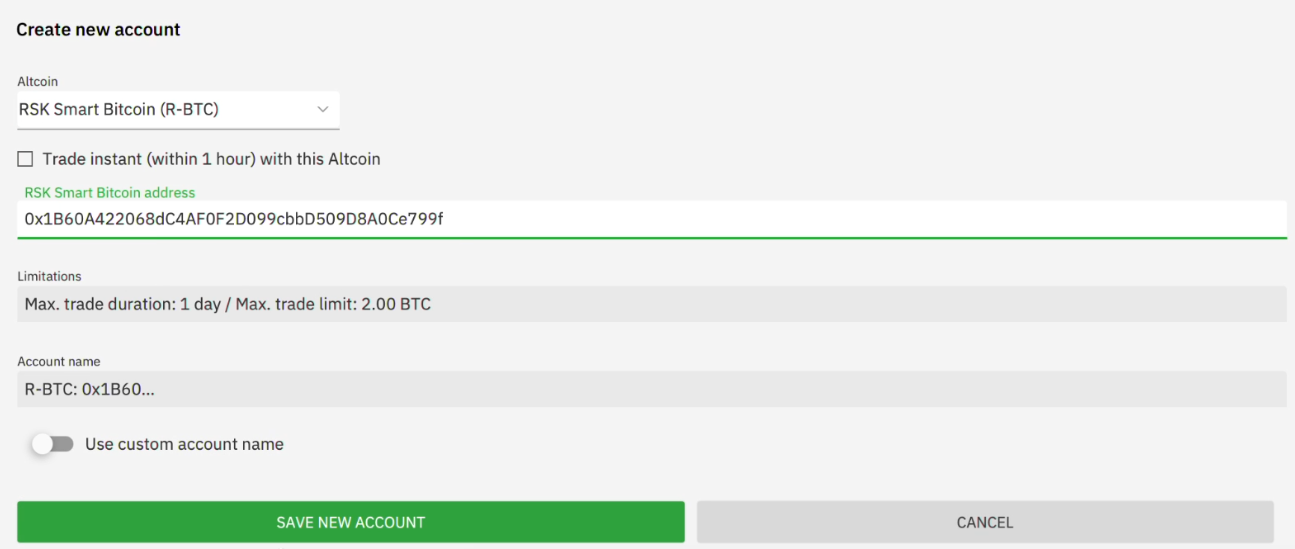
\includegraphics[page=1,height=3cm]{img/bisq-support-for-rbtc}\\
  \small{Bisq Support for rBTC}
}

\frame{\frametitle{Bisq and the RSK Sidechain}
  \centering
  
  You can see a video demonstrating Bisq Support for rBTC at:
  
  \url{https://youtu.be/dEkF6RHYx18?t=17}
}

\section{The Cost of Liquidity}

\frame{\frametitle{The Cost of Liquidity}
  \begin{itemize}
    \item Suppose you have BTC and rBTC, and you want to provide liquidity to the system.
    \item You can:
    \begin{enumerate}
      \item Make offers on Bisq to buy and sell rBTC for BTC.
      \item Occassionally, peg-in to exchange BTC for rBTC.
      \item Occassionally, peg-out to exchange rBTC for BTC.
    \end{enumerate}
  \end{itemize}
}

\frame{\frametitle{The Cost of Liquidity}
  \centering
  
  \begin{columns}
    \column{0.3\linewidth}

    \underline{\textbf{Make an Offer}}

    \column{0.3\linewidth}

    \underline{\textbf{Peg-In}}

    \column{0.3\linewidth}

    \underline{\textbf{Peg-Out}}
  \end{columns}

  \vspace{0.5cm}

  \begin{columns}
    \column{0.3\linewidth}

    BSQ Trade Fee $+$\\
    BTC Mining Fee

    \column{0.3\linewidth}

    BTC Mining Fee

    \column{0.3\linewidth}

    RSK Mining Fee $+$\\
    BTC Mining Fee
  \end{columns}

  \vspace{0.5cm}

  \begin{columns}
    \column{0.3\linewidth}

    \num{11.45}~BSQ/BTC $+$\\
    \num{239}~vB tx

    \column{0.3\linewidth}

    \num{163}~vB tx

    \column{0.3\linewidth}

    44k gas $+$\\
    \num{1074}~vB tx
  \end{columns}

  \vspace{0.5cm}

  \begin{columns}
    \column{0.3\linewidth}

    \$\num{14.15}/BTC $+$\\
    \$\num{2.36}

    \column{0.3\linewidth}

    \$\num{1.61}

    \column{0.3\linewidth}

    \$\num{0.09} $+$\\
    \$\num{10.63}
  \end{columns}

  \vspace{0.5cm}
  
  \small{@ \num{3746}~sat/BSQ, \num{30}~sat/vB, \num{0.06}~gwei, \num{33000}~\$/BTC}
}

\frame{\frametitle{The Cost of Liquidity}
  Additionally,
  \begin{itemize}
    \item The party selling rBTC also needs to mine an additional transaction to send the rBTC.
    \item The taker of a Bisq offer needs to mine three additional Bitcoin transactions to complete the trade.
  \end{itemize}
  
  \centering
  
  \textbf{Also, a peg-out transaction currently pays approximately twice the fee market rate!}
}

\section{Bisq as an Alternative}

\frame{\frametitle{Bisq as an Alternative}
  Converting between BTC and rBTC using Bisq has a number of benefits:
  \begin{itemize}
    \item While Bisq trades are somewhat more expensive than pegging in, they can also be much faster.
    \item Pegging out is more expensive than peggings in, and for conversions of less than \num{0.65} BTC, Bisq is a cheaper alternative.
    \item Bisq trades often pay BTC mining fees at below market rate, currently as low as 8.8 sat/vB.
  \end{itemize}
}

\begin{frame}[standout]
  \centering
  That's it!
\end{frame}

\end{document}
